\chapter{$ISA^{2}$}

Hemos hablado en la introducción sobre las soluciones \ac{ISA} a grandes rasgos y la principal novedad de $ISA^{2}$ frente a éstas. En este capítulo vamos a comenzar revisando el estado del arte (Sección \ref{sec:isa2_estado_del_arte}, destacando trabajos relacionados en el ámbito de las soluciones \ac{ISA}. En la Sección \ref{isa2_model}, detallaremos el sistema $ISA^{2}$ sobre el que hemos trabajado en este proyecto. Finalmente, la Sección \ref{isa2_modelo_nuevo} incluye la descripción de los cambios que hemos implementado sobre el sistema original para hacerlo más rápido y eficaz.


\section{Trabajos relacionados}
\label{sec:isa2_estado_del_arte}
%TODO: Añadir una revisión del estado del arte en tecnología ISA. Describir primero soluciones comerciales, y cómo funcionan. Luego añadir otro párrafo de soluciones que se basen en imágenes o que sean papers que soluiones el problema. Puedes traducir y reescibir de nuevo la sección del estado del arte del paper de ISA^2.

\section{El modelo $ISA^{2}$}
\label{isa2_model}

En esta sección vamos describir cómo funciona todo el sistema $ISA^{2}$, centrándonos en cada parte que lo compone para que resulte más fácil su comprensión. He aquí unas figuras ilustrativas que nos servirán como punto de referencia durante todo el capítulo.


\begin{figure}[H]
  \centering
  \includegraphics[width=8cm]{Figuras/Figura_Esquema_ISA2_Version_1_SegSem.eps}
  \caption{Esquema $ISA^{2}$ Antiguo}
  \label{fig:Isa_v1}
\end{figure}

Como se puede ver al pie de la figura \ref{fig:Isa_v1}, este fue el esquema utilizado para la primera versión de $ISA^{2}$, publicada en \cite{isa2}, cuyo funcionamiento pasamos a detallar.
%TODO: No lo hagas con item, hay que hacerlo con párrafos extensos, donde puedas resumir todo el artículo del ISA^2. Ya te anticipo que faltan bastantes detalles. El TFG no es un diario de trabajo, es un documento técnico, donde debes demostrar soltura, y reflejar los conocimientos que has aprendido.


En primera instancia el sistema recogía un set de imágenes que se correspondía con situaciones de tráfico, tanto en autovía (o autopista) como en núcleos urbanos. En concreto, la base de datos que se ofrece en \cite{isa2} \dots %TODO: añade detalles de las secuencias, número de imágenes, figura con las mismas, etc.

Para cada imagen de la base de datos se dispone de la anotación de la velocidad a la que el vehículo debe de circular. Este proceso de anotación se hizo dándo indicaciones a los conductores que participaron de la adquisición de las secuencias de vídeo mientras conducían. Así pues, se dispone de una base de datos con imágenes y velocidades asociadas, que se empleó para entrenar soluciones de inteligencia artificial y visión computador, que fuesen capaces de realizar una regresión, para una imagen de entrada, de la velocidad a la que debía circular el vehículo. A continuación pasamos a describir todos los detalles de la implementación presentada en \cite{isa2}.

%TODO: Empieza a dar más detalles técnicos de todas las partes del sistema. Hay que explicar todo.
El sistema comienza realizando una \ac{SS} de la imagen de entrada. La \ac{SS} es un proceso por el cual los píxeles de una imagen son dotados de distintos valores para poder diferenciarlos en etiquetas unos de otros y así reconocer los elementos que componen dicha imagen \cite{deeplab}. 

%TODO: añade imagen con segmentación semántica y laimagen sin segmentar, y adaptas el texto de este párrafo que de dejo comentado.
%Por ejemplo: Una fotografía de una persona, un coche y un perro. A priori, todos los píxeles de la imagen no están categorizados y no se sabe qué partes de la imagen corresponden a la persona, al coche, y al perro. Gracias a la segmentación semántica los píxeles de la imagen adquieren los valores de las etiquetas referentes a \textbf{persona}, a \textbf{coche} y a \textbf{perro}; y son fácilmente distinguibles entre sí. 

Para la \ac{SS}, el modelo en \cite{isa2} empleó la arquitectura conocida como \textbf{DeepLab} \cite{deeplab}. \textbf{DeepLab} necesita recibir como entrada la imagen en diferentes escalas. Este modelo tenía como base una \ac{CNN}, es decir, una \textbf{Red Neuronal Convolucional} \cite{cnn}. %TODO: falta una breve descripción del modelo. Un párrafo es suficiente.
 

%TODO: Falta convertir estos item en párrafos como yo he hecho con el primero. Hay que explicar cada paso en detalle: los histogramas, las pirámides (qué son?, niveles?, cómo se computan?), los modelos de regresión que se probaron, etc.
%\item Tras este proceso, mediante unos códigos de \textbf{Matlab} se recogían los datos de los píxeles ya segmentados y se organizaban en histogramas. Basándonos en los histogramas generados, usábamos una estrategia llamada \ac{SPP} \cite{spp} para crear un descriptor de imagen.

%\item Por último, el descriptor generado en el paso anterior se pasaba a diferentes sistemas de regresión. Para cada uno de ellos se añadía \ac{SI} \cite{spp} usando \ac{SPP} de hasta 3 niveles para poder compararlos entre sí y saber cuál era mejor. Para ello cogíamos los mejores resultados de cada sistema entre todos los niveles usados, y los usábamos como referencia.





%TODO: toda esta subsección hay que moverla al capítulo de resultados, donde explicas la métrica
\subsection{mIoU}

Para saber qué porcentaje de acierto ha tenido el proceso de segmentación semántica utilizaremos la métrica conocida como \ac{mIoU} \cite{miou-iou}. Esta métrica se basa en hacer la media de la \ac{IoU} de las diferentes etiquetas de clases.

La \ac{IoU} \cite{miou-iou} es la relación de superposición que existe entre la imagen segmentada y la original. Es decir, sirve para dictaminar con cuánta precisión se ha realizado el proceso de \ac{SS}. En las siguientes figuras se puede ver un ejemplo muy práctico:

\begin{figure}[H]
  \centering
  \includegraphics[width=8cm]{Figuras/Iou_1.eps}
  \caption{Imagen Original}
\end{figure}

\begin{figure}[H]
  \centering
  \includegraphics[width=8cm]{Figuras/IoU_2.eps}
  \caption{Predicción}
\end{figure}

\section{Propuesta de modelo $ISA^{2}$ mejorado}
\ref{isa2_modelo_nuevo}
El trabajo fundamental de este TFG ha consistido en mejorar el sistema tradicional $ISA^{2}$. Nuestro objetivo con este TFG es el de conseguir un sistema $ISA^{2}$  que pueda funcionar en tiempo real, y que consuma pocos recursos de GPU, para poder ser embebido en una plataforma de procesado dentro de un vehículo inteligente. La solución descrita en \cite{isa2} no cumplía ninguno de estos requisitos, principalmente por el sistema DeepLab que llevaba integrada. DeepLab es un modelo que da excelentes prestaciones en cuanto a segmentación semántica se refiere, pero no funciona en tiempo real, y además necesita una tarjeta de procesado con mucha memoria de GPU y muy alto consumo.
%TODO: Sigue motivanto tú el trabajo, saca información del artículo siftwnet. en la intro se ve que hay familias de modelos que funcionan en real-time, ventajas, inconvenientes.


En resumen, para conseguir un modelo $ISA^{2}$ más rápido y eficaz, hemos decidido cambiar el sistema de segmentación semántica Deeplab por el conocido como \textbf{Swiftnet} \cite{swiftnet}. La idea puede verse reflejada en la Figura \ref{fig:Isa_v2}.

\begin{figure}[H]
  \centering
  \includegraphics[width=8cm]{Figuras/Figura_Esquema_ISA2_Version_2.eps}
  \caption{Esquema $ISA^{2}$ Actual}
    \label{fig:Isa_v2}
\end{figure}


Como se puede comprobar, el esquema de la figura \ref{fig:Isa_v2} sigue el mismo camino que el de la primera versión, salvo por unas modificaciones al principio que pasamos a explicar a continuación:

\begin{enumerate}

\item Las imágenes de entrada al modelo de \ac{SS} no llegan en diferentes escalas como se podría intuir. La razón de por qué es así es Swiftnet: El modelo admite tanto imágenes en diferentes escalas como imágenes con una única escala. Sin embargo, para este proyecto hemos optado por la recomendación de los autores \cite{github_swiftnet} y hemos decidido hacerlo con una única escala. De esta manera hemos obtenido los resultados esperados con la base de datos de \textbf{Cityscapes} \cite{cityscapes} que ellos mismos utilizaron \cite{swiftnet}.

\item La segunda, y última, modificación es la más obvia: la sustitución del modelo de DeepLab \cite{deeplab} por el modelo de Swiftnet \cite{swiftnet}. A diferencia del primero, Swiftnet es un modelo que opera en tiempo real (\textbf{Real-Time}) de tal modo que cuando procesa una imagen lo hace en el momento, a una tasa de %TODO: añade la velocidad a la que funciona en frames por segundo, seguro que viene en el paper original de siftnet.

\end{enumerate}


En el siguiente capítulo hablaremos acerca de la implementación de Swiftnet y de cómo es mejor para los campos de aplicación, especificados anteriormente, con respecto a DeepLab.
